\subsection{Study Evaluation} \label{subsec:evaluation}
% Proofing out setup with cancer-associated genes
% chosen algorithm - Pagerank
% chosen measure - Delta TPM
% chosen Dataset

% Checking Cancer-Associated Genes
\subsubsection*{Evaluation of the Network with cancer-associated Genes} \label{subsubsec:evaluation_known_genes}
To evaluate the robustness of our network construction and PageRank algorithm,
we assess the placement of genes known to be involved in cancer development within our network.
Specifically, we examined a set of 9 genes identified as being associated with lung cancer
in a study by El-Telbany et al.~\cite{ElTelbany2012LungCancerGenes}.
We sought to determine whether these cancer-associated genes would emerge as hub nodes or exhibit high PageRank scores,
and how their expression levels $\Delta_{TPM}$ compare to those of other genes within our network.

We found that all 9 genes are present in our network,
which is a positive validation of the comprehensive coverage of our dataset.
Notably, the gene LKB1 is listed under the name STK11 in our data, which is a common alias for this gene.
\cref{fig:05_01_df_known_genes} provides an illustration of these genes
and their respective $\Delta_{TPM}$ values and PageRank scores.

\begin{figure}[!h]
    \centering
    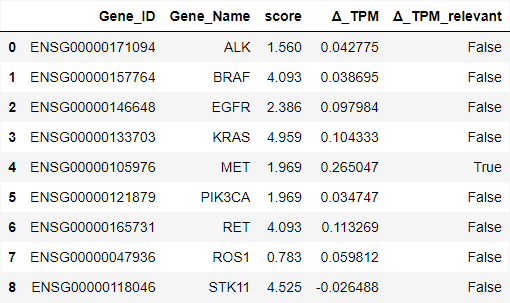
\includegraphics[height=\dfheightdouble]{figures/05_01_df_known_genes}
    \caption{9 known cancer-associated genes and their respective $\Delta_{TPM}$ values and PageRank scores}
    \label{fig:05_01_df_known_genes}
\end{figure}

When examining the placement of these cancer-associated genes within the network,
we observed that only one gene (with a $\Delta_{TPM}$ value of 0.265) is classified as $delta TPM relevant$.
None of the others have a notable $\Delta_{TPM}$ value,
with most being situated in the middle of the distribution and showing no clear pattern or outliers.

Upon examining the placement of these cancer-associated genes, we observed that none of them have a pagerank score greater than 5,
which seems to be far away from the top 10 genes.
However, as shown in \cref{fig:05_known_genes},
4 of the 9 genes are situated within the top 10 percent of the distribution (PR score \> 3.67),
and all are above the median, indicating that they are relatively well-connected nodes within our network.

\begin{figure}[h]
    \minipage{0.45\textwidth}
        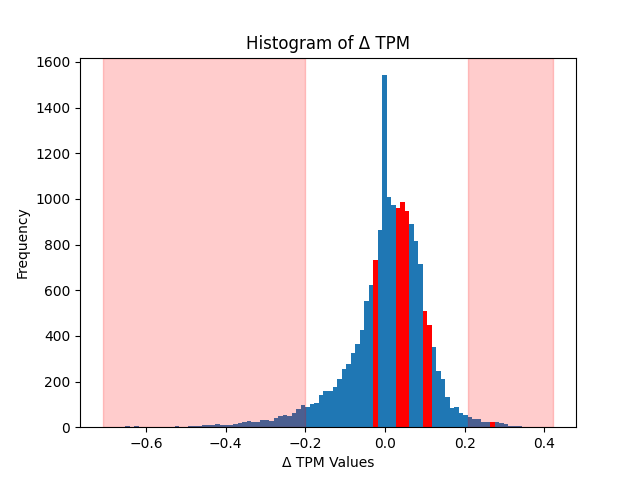
\includegraphics[width=\linewidth]{figures/05_01_delta_tpm_relevant}
    \endminipage
    \hfill
    \minipage{0.45\textwidth}
      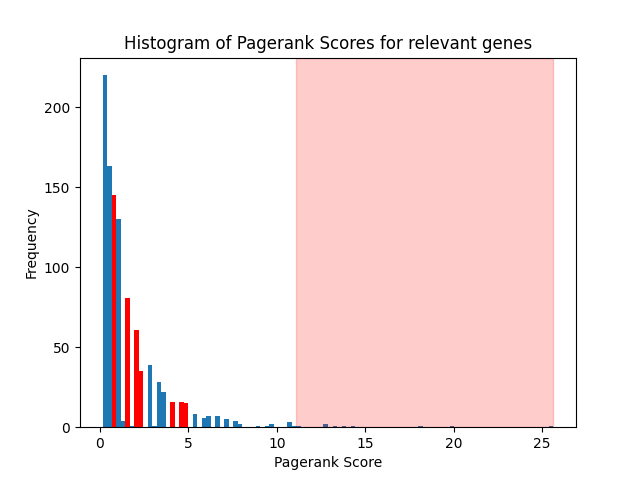
\includegraphics[width=\linewidth]{figures/05_01_pagerank_known_genes}
    \endminipage
    \caption{Distribution of the Pagerank score and the $\Delta_{TPM}$ with highlighting of values for 9 known cancer-associated genes}
    \label{fig:05_known_genes}
\end{figure}

Our analysis suggests that while our network construction and PageRank algorithm are robust,
the placement of these cancer-associated genes within the network may not be directly indicative
of their role in cancer development.\\
% TODO longer

%%%%%%%%%%%%%%%%%%%%%%%%%%%%%%%%%%%%%%%%%%%%%%%%%%%%%%%%%%%%%%%%%%%%%%%%%%%%%%%%%%%%%%%%%%%%%%%%%%%%%%%%%
% Delta TPM relevant
\subsubsection*{Limitation of the $\Delta_{TPM}$ and the $\Delta TPM relevant$ measure} \label{subsubsec:limit_delta_tpm}
The calculated $\Delta_{TPM}$ values represent the relative difference in gene expression between normalized mean cancerous and healthy states,
indicating an increase or decrease in transcript abundance in the tumor compared to normal tissue.
We classified the significant 5\% of the genes as $\Delta TPM relevant$ in our study.

The top 10 genes that we looked at all had a connection to cancer based on previous studies
- even if not all of them had a connection to lung cancer.
However, 10 genes is a rather small group to make a general statement of the quality of the delta TPM measure we developed.
By looking at the genes known for lung cancer, only one was classified as having relevant changes in gene activity.
This raises questions about the robustness and sensitivity of our approach.
While it seems like a solid starting point, there are some limitations and improvements that could be made based on the assumptions we made.

% what can be criticized? And how can it be improved?
One potential problem may be that our calculation assumes a linear relationship between healthy and cancerous TPM values
by subtracting the log-scaled mean TPM values.
Additionally, the log-scaled normalization method of TPM values might not be optimal,
and could be improved by using a different, e.g. non-linear method such as quantile normalization.
Furthermore, our measure may be too general, potentially leading to false negatives for genes that are more sensitive to smaller changes.
To address these concerns, it could be a way to investigate the correlation between xxx with methods like fold change and enrichment scores.
Another improvement could be to use an additional measure such as FPKM or RPKM to validate the TPM results and not rely on only one measure.
\\

%%%%%%%%%%%%%%%%%%%%%%%%%%%%%%%%%%%%%%%%%%%%%%%%%%%%%%%%%%%%%%%%%%%%%%%%%%%%%%%%%%%%%%%%%%%%%%%%%%%%%%%%%
% PageRank
\subsubsection*{Limitation of the PageRank score} \label{subsubsec:limit_pagerank}
% How did it work?
We calculated the PageRank score for each gene in our network to determine its importance within the network
and find the most influential genes based on their connections.

% Did it work well?
As expected the distribution of the Pagerank scores was logarithmic / exponential with a few genes having a high score and most genes having a low score.
Since

% Improve Ideas
% Zu viel Gewicht auf den ersten Edges? Quasi nur abhängig von Anzahl der Kanten am Gen - da hätte man sich den Pagerank sparen können
% It seems that the PageRank score is heavily influenced by the number of proteins a gene transcribes.
% Meaning the number of first level edges a gene has in the network.
% This could be because the number of second level edges (connections from a protein to another protein) is very constant.
% If this is the case the PageRank score is not really needed as we could have just counted the number of proteins a gene transcribes.

% TODO plot the distribution of interactions by protein





% inital Data
\subsubsection*{Limitation of the used base datasets} \label{subsubsec:limit_base_data}
* Other datasets could be used like TCGA which is common in cancer research
* CMP Dataset matched with ENS ID Names might be wrong - would be better to find a good dataset with ens IDs

% Verallgemeinerung der Daten
% gibt keine Inforamtion über Ethnie
% Especially the focus on the older age range may affect the generalizability of our findings to other populations.


